\begin{figure}
	\centering
	\makebox[\textwidth][c]{
		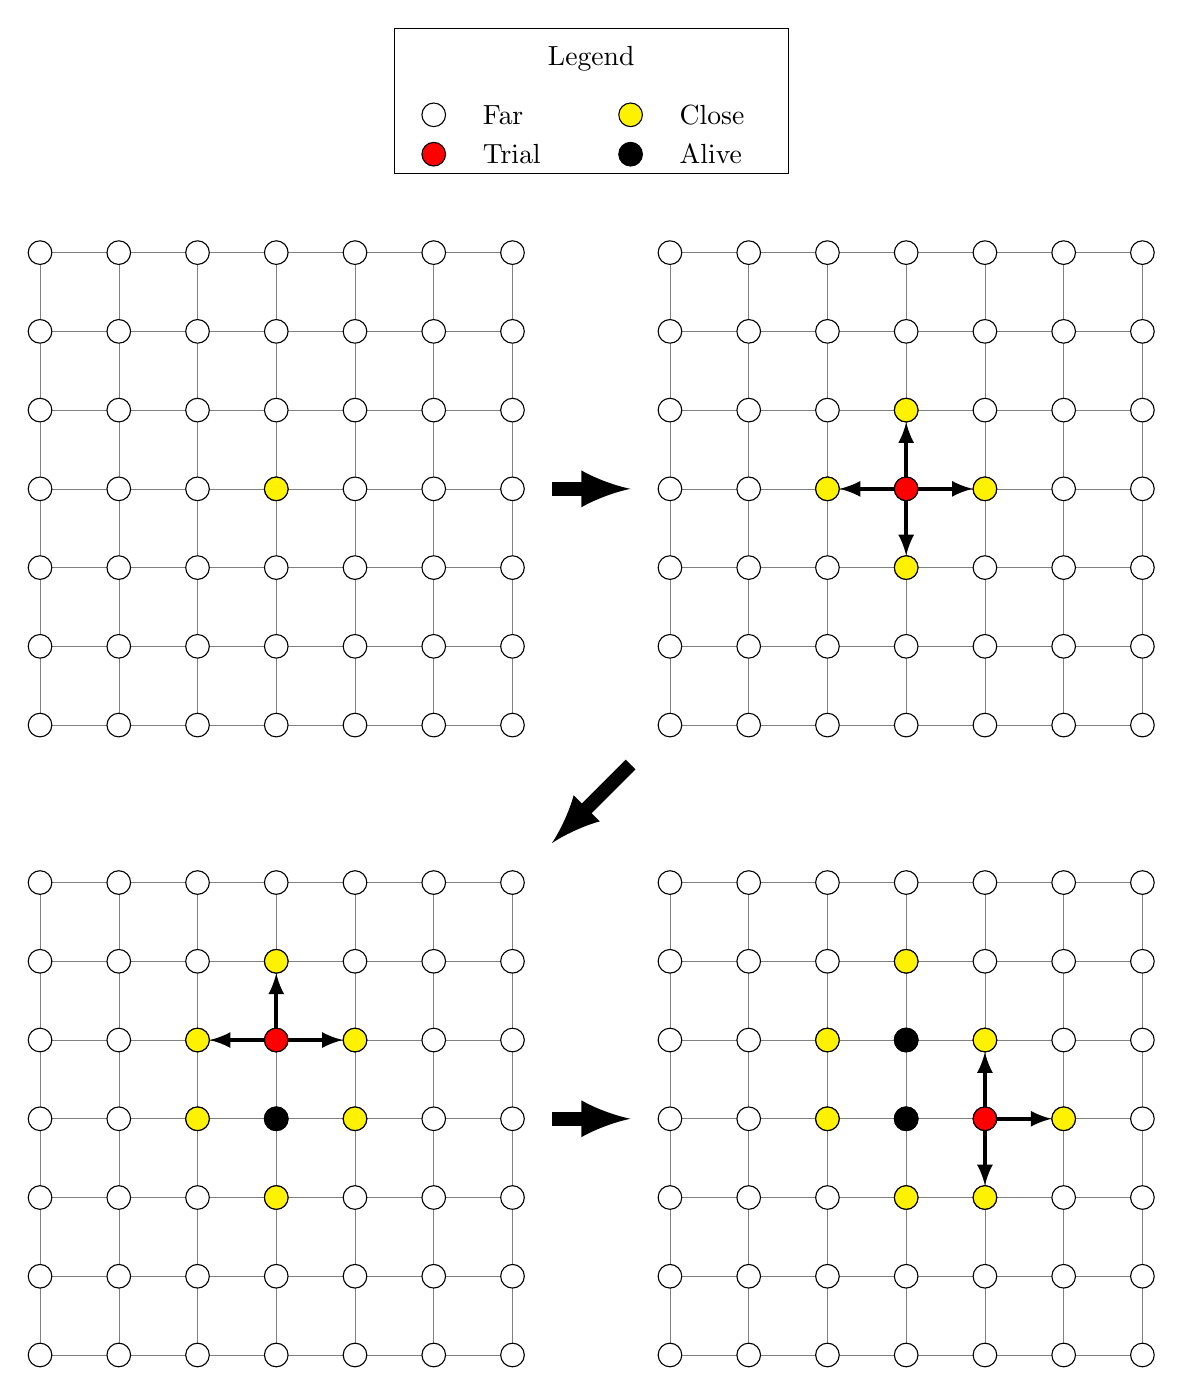
\begin{tikzpicture}[axis/.style={thin, black, ->, >=stealth'}]
			
			\def \radius{0.15}
			\def \cfar{white}
			\def \cclose{yellow}
			\def \ctrial{red}
			\def \calive{black}
			
			\draw (4.5, 15) rectangle (9.5, 16.85);
			\node[align=left,anchor=north] at (7, 16.75) {Legend};
			\filldraw[fill=\cfar]             (5,  15.75) circle (\radius);
			\node[align=left,anchor=west] at  (5.5,15.75) {Far};	
			\filldraw[fill=\cclose]           (7.5,  15.75) circle (\radius);
			\node[align=left,anchor=west] at  (8,    15.75) {Close};
			
			\filldraw[fill=\ctrial]           (5,  15.25) circle (\radius);
			\node[align=left,anchor=west] at  (5.5,15.25) {Trial};
			
			\filldraw[fill=\calive]           (7.5,15.25) circle (\radius);
			\node[align=left,anchor=west] at  (8,  15.25) {Alive};
	
			% GRID A
			\def \xmin{0}
			\def \xmax{6}
			\def \ymin{8}
			\def \ymax{14}
			\draw[step=1cm,gray,very thin] (\xmin, \ymin) grid (\xmax, \ymax);
			\foreach \ix in {\xmin,...,\xmax}{
				\foreach \iy in {\ymin,...,\ymax}{
					\filldraw[fill=\cfar] (\ix,\iy) circle (\radius);
				}
			}
			\filldraw[fill=\cclose] (\xmin+3,\ymin+3) circle (\radius);
			
			\draw[-latex,line width=5pt] (\xmax+0.5, \ymin+3) -- (\xmax+1.5, \ymin+3);
			
			% GRID B
			\def \xmin{8}
			\def \xmax{14}
			\def \ymin{8}
			\def \ymax{14}
			\draw[step=1cm,gray,very thin] (\xmin, \ymin) grid (\xmax, \ymax);
			\foreach \ix in {\xmin,...,\xmax}{
				\foreach \iy in {\ymin,...,\ymax}{
					\filldraw[fill=\cfar] (\ix,\iy) circle (\radius);
				}
			}
			\filldraw[fill=\ctrial] (\xmin+3,\ymin+3) circle (\radius);
			\filldraw[fill=\cclose] (\xmin+3,\ymin+4) circle (\radius);
			\filldraw[fill=\cclose] (\xmin+3,\ymin+2) circle (\radius);
			\filldraw[fill=\cclose] (\xmin+4,\ymin+3) circle (\radius);
			\filldraw[fill=\cclose] (\xmin+2,\ymin+3) circle (\radius);
	
			\draw[-latex,ultra thick] (\xmin+3, \ymin+3+\radius) -- (\xmin+3, \ymin+4-\radius);
			\draw[-latex,ultra thick] (\xmin+3, \ymin+3-\radius) -- (\xmin+3, \ymin+2+\radius);
			\draw[-latex,ultra thick] (\xmin+3+\radius, \ymin+3) -- (\xmin+4-\radius, \ymin+3);
			\draw[-latex,ultra thick] (\xmin+3-\radius, \ymin+3) -- (\xmin+2+\radius, \ymin+3);
			
			\draw[-latex,line width=5pt] (\xmin-0.5, \ymin-0.5) -- (\xmin-1.5, \ymin-1.5);
			
			% GRID C
			\def \xmin{0}
			\def \xmax{6}
			\def \ymin{0}
			\def \ymax{6}
			\draw[step=1cm,gray,very thin] (\xmin, \ymin) grid (\xmax, \ymax);
			\foreach \ix in {\xmin,...,\xmax}{
				\foreach \iy in {\ymin,...,\ymax}{
					\filldraw[fill=\cfar] (\ix,\iy) circle (\radius);
				}
			}
			\filldraw[fill=\calive] (\xmin+3,\ymin+3) circle (\radius);
			\filldraw[fill=\ctrial] (\xmin+3,\ymin+4) circle (\radius);
			\filldraw[fill=\cclose] (\xmin+3,\ymin+2) circle (\radius);
			\filldraw[fill=\cclose] (\xmin+4,\ymin+3) circle (\radius);
			\filldraw[fill=\cclose] (\xmin+2,\ymin+3) circle (\radius);
			\filldraw[fill=\cclose] (\xmin+3,\ymin+5) circle (\radius);
			\filldraw[fill=\cclose] (\xmin+4,\ymin+4) circle (\radius);
			\filldraw[fill=\cclose] (\xmin+2,\ymin+4) circle (\radius);
			
			\draw[-latex,ultra thick] (\xmin+3, \ymin+4+\radius) -- (\xmin+3, \ymin+5-\radius);
			\draw[-latex,ultra thick] (\xmin+3+\radius, \ymin+4) -- (\xmin+4-\radius, \ymin+4);
			\draw[-latex,ultra thick] (\xmin+3-\radius, \ymin+4) -- (\xmin+2+\radius, \ymin+4);
			
			\draw[-latex,line width=5pt] (\xmax+0.5, \ymin+3) -- (\xmax+1.5, \ymin+3);
			
			% GRID D
			\def \xmin{8}
			\def \xmax{14}
			\def \ymin{0}
			\def \ymax{6}
			\draw[step=1cm,gray,very thin] (\xmin, \ymin) grid (\xmax, \ymax);
			\foreach \ix in {\xmin,...,\xmax}{
				\foreach \iy in {\ymin,...,\ymax}{
					\filldraw[fill=\cfar] (\ix,\iy) circle (\radius);
				}
			}
			\filldraw[fill=\calive] (\xmin+3,\ymin+3) circle (\radius);
			\filldraw[fill=\calive] (\xmin+3,\ymin+4) circle (\radius);
			\filldraw[fill=\cclose] (\xmin+3,\ymin+2) circle (\radius);
			\filldraw[fill=\ctrial] (\xmin+4,\ymin+3) circle (\radius);
			\filldraw[fill=\cclose] (\xmin+2,\ymin+3) circle (\radius);
			\filldraw[fill=\cclose] (\xmin+3,\ymin+5) circle (\radius);
			\filldraw[fill=\cclose] (\xmin+4,\ymin+4) circle (\radius);
			\filldraw[fill=\cclose] (\xmin+2,\ymin+4) circle (\radius);
			\filldraw[fill=\cclose] (\xmin+5,\ymin+3) circle (\radius);
			\filldraw[fill=\cclose] (\xmin+4,\ymin+2) circle (\radius);
			
			\draw[-latex,ultra thick] (\xmin+4, \ymin+3+\radius) -- (\xmin+4, \ymin+4-\radius);
			\draw[-latex,ultra thick] (\xmin+4+\radius, \ymin+3) -- (\xmin+5-\radius, \ymin+3);
			\draw[-latex,ultra thick] (\xmin+4, \ymin+3-\radius) -- (\xmin+4, \ymin+2+\radius);
			
	
		\end{tikzpicture}
	}
	\caption{A 2D illustration of the update scheme (Algorithm \ref{alg:fmm_update}) used by the FMM}
	\label{fig:fmm_update}
\end{figure}